\chapter{Observational Constraints on PBH Abundance }


PBHs are crucial to our understanding of the universe.
They can produce a variety of observed effects that are directly caused by their gravitational potential and are therefore unrelated to the processes that led to the formation of PBHs. This allows us to constrain their current abundance. This section will address several constraints for PBHs that haven't completely evaporated yet and briefly discuss the upper limit for the PBH fraction in dark matter.
We will first discuss the constraints under the assumption that the PBH mass function is monochromatic, i.e., $\Delta M \sim M$, which is valid when the width of the mass function is sufficiently narrow. The fraction $f(M)$ of the halo in PBHs is related to $\beta(M)$ as given in Eq. \ref{3.14}. However, as we discussed in section \ref{limtiation}, in many cases, the PBH is expected to produce an extended mass distribution, which requires separate analysis. We will briefly discuss this in sections \ref{emd}, for more  details Ref. \cite{Carr:2016drx, Carr:2017jsz, Green:2016xgy, Bellomo:2017zsr} can be referred to. The sections following will cover the key constraints. Although the limits that will be outlined can't be applied to every potential PBH scenario, they are nevertheless useful in excluding some of them. The constraints on the contribution of PBH to dark matter, further discussion on claimed signature and viable mass windows Ref.\cite{Sasaki_2018, Carr:2019kxo, Carr:2020xqk} can be referred.\\

\begin{figure}[h]
    \centering
    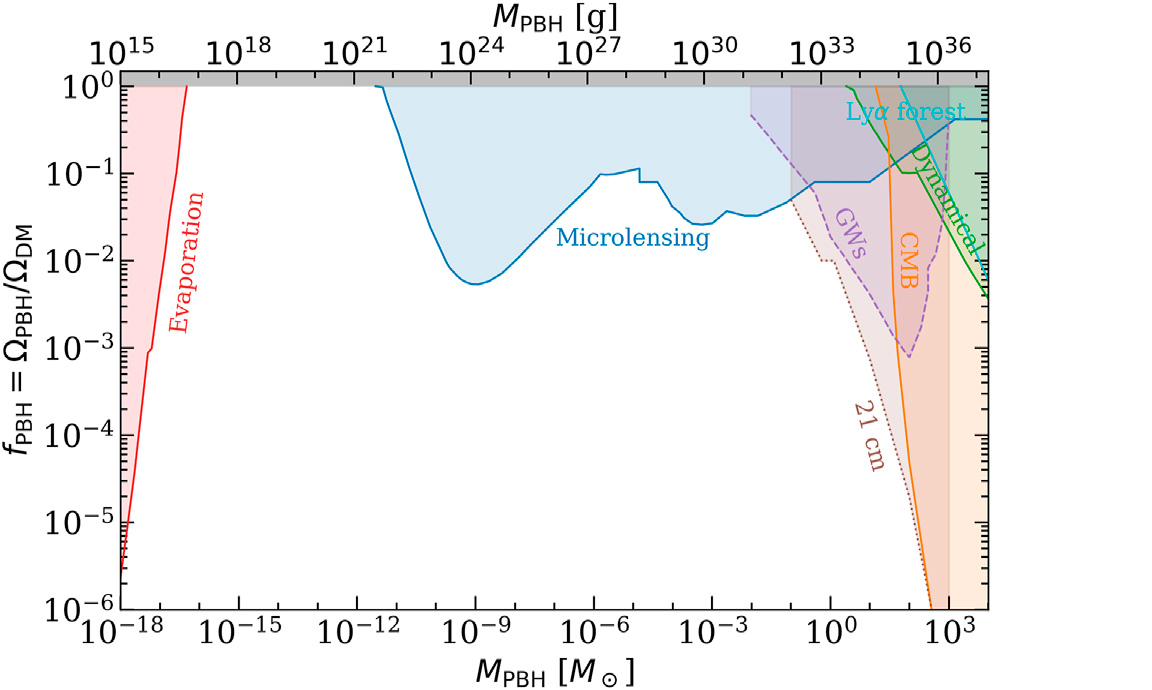
\includegraphics[width=0.7\textwidth]{Constraints.png}
    \caption{Compilation of constraints on the PBH fraction (with respect
to DM) as a function of the PBH mass, assuming a monochromatic mass
function. Impact of PBH evaporation(red) on the extragalactic $\gamma$-ray background  and on the CMB spectrum. Non-observation of microlensing events
(blue) from the MACHO, EROS, Kepler, Icarus, OGLE,  and Subaru-HSC collaborations. PBH accretion signatures on the CMB (orange), assuming spherical accretion of PBHs within
halos. Dynamical constraints, such as disruption of stellar
systems by the presence of PBHs (green), on wide binaries and on ultra-faint dwarf galaxies.
Power spectrum from the Ly$\alpha$ forest (cyan). GW limits are denoted by dashed lines since they could be invalidated \cite{2021JCAP...03..078B}. The dotted brown line corresponds to forecasts from the 21 cm power spectrum with SKA sensitivities \cite{Mena:2019nhm} and from 21 cm forest prospects. Figure is taken from \cite{Villanueva-Domingo:2021spv}}
    \label{fig:4.1} 
\end{figure}


%%%%%%%%%%%%%%%%%%%%%%%%%%%%%%%%%%%%%%%%%%%%%%%%%%%%%%%%%%%%%%%%%
\section{Evaporation Constraints}
In the year 1974, Hawkings\cite{1974Natur.248...30H} \cite{Hawking:1975vcx} claimed the possibility of black holes emitting radiation due to the process of pair creation and annihilation at the event horizon. A black hole emits thermal radiation with temperature
\begin{align}
      T = \frac{\hbar c^{3}}{8\pi G M k_{B}} \simeq 10^{-7} \qty(\frac{M}{M_{\odot}})^{-1} \mathrm{K} \label{4.1}
\end{align}
  
where $k_{b}$ is the Boltzmann's constant , $\hbar$ is the reduced Placks constant, $G$ is the graviational constant and $c$ is the speed of light. Let us find the time taken for a black hole to evaporate from the Stefan Boltzmann law.
\begin{align}
    P = \sigma A T^4 \label{4.2}
\end{align}
where $A = 4 \pi R_{s}^2$ and $T$ is the temperature. The power radiated is the rate of energy loss from the black hole i.e. $P = -c^2 \dv{M}{t}$. Using this equation \ref{4.2}, substituting \ref{4.1} and integrating from $M$ at $t=0$ to $M=0$ at $t = \tau$  we find the relation between the mass of the black hole and its lifetime as
\begin{align}
   \tau(M) \simeq \frac{\hbar c^4}{G^2 M^3} \simeq 10^{64} \left(\frac{M}{M_{\odot}}\right)^{3} \mathrm{yrs} \label{4.3}
\end{align}

Since the lifetime of the Universe is $1.3 \times 10^{10}$ years, $ (\frac{M}{M_{\odot}})^3   \simeq 1.38 \times  10^{54}$ and $(M/M_{\odot}) \simeq  1.11 \times 10^{18}$. Given that$M_{\odot} = 2 \times 10^{30}$ kg, only black holes smaller than about $10^{12}$ kg would have evaporated by the present epoch, so Eq. \ref{3.10} suggests that this effect is only significant for black holes which formed before 1$0^{-23}$s. $M < M_{*} \approx 5\times 10^{14}g $ will already have been evaporated  by the Hawking radiation. The observations of the extra-galactic $\gamma$-ray background put up a strong constraint on $f(M_{*})$. Although those in the narrow mass range $M_{*} < M < 1.005 M_{*}$ have not yet finished evaporating, their present mass is less than the mass $M_q \approx 0.4 M_{*}$ at which quark and gluon jets are released. The time-integrated spectrum of photons from each PBH is derived by multiplying the instantaneous spectrum by the age of the Universe $t_0$ for $M > 2 M$, where it is possible to completely disregard the change in mass. The instantaneous spectrum for primary photons is given by
\begin{align}
    \frac{\mathrm{d} \dot{N}_\gamma^{\mathrm{P}}}{\mathrm{d} E}(M, E) \propto \frac{E^2 \sigma(M, E)}{\exp (E M)-1} \propto \begin{cases}E^3 M^3 & \left(E<M^{-1}\right) \\ E^2 M^2 \exp (-E M) & \left(E>M^{-1}\right)\end{cases} \label{4.4}
\end{align}

where $\sigma(M, E)$ is the absorption cross-section for photons of energy $E$, so this gives an intensity
\begin{align}
    I(E) \propto f(M) \times \begin{cases}E^4 M^2 & \left(E<M^{-1}\right) \\ E^3 M \exp (-E M) & \left(E>M^{-1}\right) .\end{cases} \label{4.5}
\end{align}

This peaks at $E^{\max } \propto M^{-1}$ with a value $I^{\max }(M) \propto f(M) M^{-2}$, whereas the observed intensity is $I^{\mathrm{obs}} \propto E^{-(1+\epsilon)}$ with $\epsilon$ between 0.1 and 0.4 , so putting $I^{\max }(M)<I^{\mathrm{obs}}[M(E)]$ gives [3]

\begin{align}
    f(M)<2 \times 10^{-8}\left(\frac{M}{M_*}\right)^{3+\epsilon} \quad\left(M>M_*\right) .\label{4.6}
\end{align}


For $\epsilon = 0.2$, the plot is shown in Figure \ref{fig:4.1}. A stronger constraint might be provided by the Galactic-ray background constraint \cite{Carr:2016hva}, but since this depends sensitively on the shape of the PBH mass function, we will not explore it here. In this mass range, there are numerous additional evaporation limitations. Boudad and Cirelli \cite{Boudaud:2018hqb} constrain evaporating PBHs of mass $M < 10^{16}$ g and get the bound $f < 0.001$ using positron data from Voyager 1. This complements the cosmological limit and is depicted in Figure \ref{fig:4.1}   as well. It is based on local Galactic measurements. Laha \cite{Laha:2019ssq} and DeRocco and Graham \cite{DeRocco:2019fjq} use observations of the 511 keV annihilation line radiation from the Galactic center to constrain $10^{16}-10^{17}$g PBHs. Additional constraints are related to measurements of the Galactic center made with radio and $\gamma$-rays \cite{Laha:2020ivk},\cite{Chan:2020zry} as well as the ionizing impact of $10^{16}-10^{17}g$ PBHs \cite{Belotsky:2014twa}.
%%%%%%%%%%%%%%%%%%%%%%%%%%%%%%%%%%%%%%%%%%%%%%%%%%%%%%%%%%%%%%%%%
\section{Lensing Constraints}
One of the major predictions of general relativity is gravitational lensing. A massive body causes spacetime to curve resulting in deflection, distortion, or magnification of light from a source that is along the line of sight of the observer.\\
In microlensing, the lens of the mass is low due to which the displacement of the light is not significant. However, the apparent brightness of the light sources changes, as the lens passes across the light source. The intensity and light curve can be used to study the lens objects which are referred to as MACHOs, which are one class of likely dark matter candidates for eg. a black hole(primordial). Microlensing events are rare, so to find them surveys of a vast region of the sky with a high number density of sources of stars are used such as the Large and Small Magellanic Clouds, the nearby Andromeda galaxy, the Milky Way bulge, etc. \\
To look for the microlensing of stars by PBHs located in the halo areas of the Milky Way and M31, Niikura \emph{et al.}\cite{Niikura:2017zjd} performed a seven-hour observation of M31 using the Subaru Hyper Suprime-Cam (HSC).
for $10^{-10}M_{\odot} < M < 10^{-6} M_{\odot}$ which is shown in Figure \ref{fig:4.1}  .
Microlensing observations of stars in the Large and Small Magellanic Clouds probe the fraction of the Galactic halo in massive compact halo objects (MACHOs) of a certain mass range \cite{1986ApJ...304...15B}. The optical depth of the halo towards LMC and SMC, which is the probability that any given star is amplified by at least 1.34 at a given time, is related to the fraction f by
\begin{equation}
    \tau_{L}^{(SMC)} = 1.4 \tau_{L}^{(LMC)} = 6.6 \times 10^{-7} f(M) \label{4.7}
\end{equation}
for the standard halo model \cite{MACHO:2000qbb}. The MACHO project detected lenses with $M \sim 0.5M_{\odot}$ but concluded that their halo contribution could be at most $10 \%$ \cite{Hamadache:2006fw}.
The EROS project gave more strict restrictions and excluded 
$ 6 \times 10^{-8}M_{\odot} < M < 15M_{\odot}$ object from dominating the halo. Further limits in the range of $ 0.1 M_{\odot} < M < 20M_{\odot} $ have come from the OGLE experiment\cite{Wyrzykowski_2009},\cite{Wyrzykowski_20111},\cite{Wyrzykowski_20112},\cite{Wyrzykowski_20113},\cite{CalchiNovati:2009kq} since then. The combined results are approximately mentioned below.\\
\begin{align}
    f(M)< \begin{cases}1 & \left(6 \times 10^{-8} M_{\odot}<M<30 M_{\odot}\right) \\ 0.1 & \left(10^{-6} M_{\odot}<M<1 M_{\odot}\right) \\ 0.05 & \left(10^{-3} M_{\odot}<M<0.4 M_{\odot}\right)\end{cases}
\end{align}
    
Recently Niikura \emph{et al.}\cite{Niikura:2019kqi} have used data from a five-year OGLE survey of the Galactic bulge to place much stronger limits in the range $10^{-6} M_{\odot}<M<10^{-4} M_{\odot}$, although they also claim some positive detections. The precise form of the EROS and OGLE limits are shown in Figure \ref{fig:4.1}  

With a long tail of high magnifications, PBHs demagnify most lines of sight compared to the mean. Zumalacárregui and Seljak \cite{Zumalacarregui:2017qqd} have exploited the lack of lensing in type Ia supernovae (SNe) to constrain any PBH population, a method that takes into account the effects of large-scale structure and potential non-Gaussianity in the intrinsic SNe luminosity distribution. Using current JLA data, they derive a bound $f<0.35$ for $10^{-2} M_{\odot}<M<10^4 M_{\odot}$, the finite size of SNe providing the lower limit, and this constraint is shown in Figure \ref{fig:4.1}. This constraint can be weakened, according to Garca-Bellido and Clesse \cite{garc2018PDU....20...95G}, if the PBHs have an extended mass function or are clustered. Although there is some disagreement on this, Figure \ref{fig:4.1}   only depicts a monochromatic mass function.\\

The recent discovery of fast transient events in massive galaxy clusters is attributed to individual stars in giant arcs being highly magnified due to caustic crossing. Oguri \emph{et al.}\cite{Oguri:2017ock} argue that the particular event MACS J1149 excludes a high density of PBHs anywhere in the mass range $10^{-5} M_{\odot}<M<10^2 M_{\odot}$ because this would reduce the magnifications.\\

Early studies of the microlensing of quasars \cite{Dalcanton1994ApJ...424..550D} seemed to exclude the possibility of all the dark matter being in objects with $10^{-3} M_{\odot}<M<60 M_{\odot}$, although this limit preceded the $\Lambda \mathrm{CDM}$ picture. More recent studies of quasar microlensing suggest a limit \cite{Mediavilla_2009} $f(M)<1$ for $10^{-3} M_{\odot}<M<60 M_{\odot}$. Millilensing of compact radio sources \cite{Wilkinson:2001vv} gives a limit

\begin{align}
     f(M)< \begin{cases}\left(M / 2 \times 10^4 M_{\odot}\right)^{-2} & \left(M<10^5 M_{\odot}\right) \\ 0.06 & \left(10^5 M_{\odot}<M<10^8 M_{\odot}\right) \\ \left(M / 4 \times 10^8 M_{\odot}\right)^2 & \left(M>10^8 M_{\odot}\right) .\end{cases}
\end{align}
   
We mention it to show that lensing limitations extend to extremely large values of $M$, despite being weaker than the dynamical constraints in this mass range and excluded from Figure \ref{fig:4.1} .\\

According to \cite{1992ApJ...386L...5G}, asteroid mass compact objects might be studied via femtolensing of $\gamma$-ray bursts (GRBs), specifically through interference fringes in the frequency spectrum caused by the two (unresolved) images' differing phases during propagation.

Assuming the bursts are at a redshift $z \sim 1$, early studies implied $f < 1$ in the mass range
$10^{-16} - 10^{-13} M_{\odot}$ \cite{Marani:1998sh}\cite{Nakamura:1997sm} and $f < 0.1$ in the range $10^{-17} - 10^{-14} M_{\odot}$ \cite{Barnacka_2012}. However, Katz \emph{et al.} \cite{Katz:2018zrn} argue that most GRB sources are too large to be modelled as point sources, and furthermore, that wave optics effects \cite{Ulmer:1994ij} need to be taken into account. Consequently, there are in fact no current constraints on f from femtolensing.




%%%%%%%%%%%%%%%%%%%%%%%%%%%%%%%%%%%%%%%%%%%%%%%%%%%%%%%%%%%%%%%%%
\section{Dynamical Constraints}
It is possible to set an upper limit on the PBH fraction for a wide range of PBH mass by appropriately analyzing the gravitational interaction influence of PBHs on astrophysical systems and comparing results with observations. Various astrophysical systems in regard to this context are discussed below (The constraints of only the former two astrophysical systems are shown in Figure \ref{fig:4.1} ).
\subsection{Ultra Faint Dwarf Galaxies}
The kinetic energies of systems with various masses often balance out and match thanks to two-body interactions. If a stellar system also has a MACHO population they  will interact with each other, which will lead to an increase in the average kinetic energy of the stars. As a result,  the system will expand because of the kinetic energy gained by the stars due virial theorem which may contradict the observed distribution of the stars. Because of the dynamic heating caused by PBHs, star clusters would eventually dissolve into their host galaxy as they became larger with higher velocity dispersions. This impact is especially pronounced in populations with high mass-to-luminosity ratios, as is the case with ultra-faint dwarf galaxies (UFDG), which would be disturbed by PBHs. Tight bounds have been obtained using these effects at $f_{\mathrm{PBH}} \sim 10^{-3}$ for $ M \sim 10^{4} M_{\odot}$\cite{Brandt:2016aco}. \\
\subsection{Wide Binaries}
Wide binary star systems may be perturbed by close encounters with compact objects, perhaps leading to disruption. The PBH fraction is constrained by the separation distribution of wide binaries from $f_{\mathrm{PBH}} \lesssim 1$ for $ M \simeq 3M_{\odot}$ to $ f_{\mathrm{PBH}} \lesssim 0.1$ at $M \gtrsim 70 M_{\odot}$ \cite{Monroy_Rodr_guez_2014}.


\subsection{Disruption of White Dwarfs}
In the event of a PBH passing inside a white dwarf, the particles inside a thin tube along the trajectory of the PBH gain energy due to the gravitational pull from the PBH for a short time. This leads to a loss in the kinetic energy of the PBH, although negligible to its initial kinetic energy which further causes an increase in the temperature of the thin tube. This increase in temperature boosts the nuclear fusion rate significantly. If the dissipation of heat from the affected region occurs faster than the timescale of nuclear fusion, fusion reactions take place, releasing energy and further increasing the temperature. In larger volumes, dissipation becomes less efficient, facilitating fusion and eventually leading to an explosion. 
Therefore, the existence of white dwarfs in the current Universe would be prevented by an overwhelming abundance of PBHs above a particular mass. On the other hand, we can limit the number of PBHs within a certain mass range by establishing the existence of white dwarfs by observation. While massive PBHs are uncommon and therefore come into contact with white dwarfs seldom, light PBHs do not exert enough gravitational pull to heat white dwarfs significantly. The fraction of PBHs as a function of their mass is therefore constrained to a maximum by this line of thinking. \cite{Graham:2015apa}


\subsection{Disruption of Neutron Stars}
Similar to white dwarfs, PBH loses kinetic energy by dynamical friction while passing through a neutron star which was studied by Ref. \cite{Capela:2013yf}. They found that the PBH becomes gravitationally bonded to the neutron star if the energy transferred from it to the neutron star is more than its original kinetic energy. Following the initial transit, the PBH goes through the neutron stars once per half oscillation period while undergoing orbital oscillations, progressively losing all kinetic energy in the process. The PBH oscillates a certain number of times before becoming trapped inside the neutron star. When this occurs, Th PBH rapidly accretes the nuclear matter and annihilates the star. The frequent exposure of neutron stars to PBH collisions must therefore be avoided. This aids in determining an upper limit on the abundance of PBH. 

\subsection{Dynamical Friction on PBHs}
Strong dynamical friction would be experienced by a PBH in the neighbourhood of the Galactic Center due to interactions with stars, lighter PBHs, and dark matter made up of elementary particles. The PBH loses kinetic energy as a result of the friction, spiralling inward towards the centre. PBH accumulation takes place in the centre of the region if the infall timescale is less than the age of the universe. As a result, either a dense cluster of PBHs or a smaller number of more massive black holes produced by merging accumulated PBHs would dominate the Galactic core. 
Given that the mass in the Galactic Center has an upper limit, this restriction can be translated into a restriction on the fraction of PBHs in the Galactic Halo within a specific mass range.\\
In reference \cite{1999ApJ...516..195C}, the constraint on the fraction of Primordial Black Holes ($f_{\text{PBH}}$) was derived by imposing a limit on the mass concentration ($M_{\text{con}}$) in the Galactic centre. Specifically, the analysis sets a restriction on $M_{\text{con}}$, such that it does not exceed the observational limit of approximately $3 \times 10^6 M_{\odot}$ on the central dark matter. This constraint is applicable for Primordial Black Holes with masses ($M_{\text{PBH}}$) greater than $4 \times 10^4 M_{\odot}$. The obtained result places a strong restriction on the abundance of PBHs within this mass range.


\subsection{Disk heating}

Primordial Black Holes (PBHs) may cross the galactic disk as they travel through the halo of the galaxy. As a result, the stars in the disk gain velocity every time a PBH approaches due to the gravitational pull between PBHs and them. The evolution of the disk stars' velocities exhibits a random walk pattern since the direction of the obtained velocity for each unique PBH passage is unpredictable. As a result, the variance of the star's velocity rises correspondingly over time, which causes the disk stars to heat up more and more.
It is possible to constrain the abundance of PBHs within a given mass range by requiring that the velocity increase brought on by PBHs does not exceed the observed velocity. This restriction takes into consideration how PBH interactions affect the distribution of stellar velocities in the Galactic disk.
(For more details refer to Ref. \cite{1999ApJ...516..195C})



%%%%%%%%%%%%%%%%%%%%%%%%%%%%%%%%%%%%%%%%%%%%%%%%%%%%%%%%%%%%%%%%%
\section{CMB Constraints}
The CMB spectrum is affected either by the radiation due to accretion or from Hawking radiation. They are affected in two ways, firstly by producing spectral distortions and secondly by modifying temperature anisotropies. The energetic radiation can increase ionization rates, delay recombination, shift the peaks of the CMB anisotropy spectrum, and cause more diffusion damping. As the Thomson optical depth and reionization bump at large angular scales would both be enhanced by an increase in the free electron fraction, the polarization spectrum might also be altered.\\
The effects of PBH on early CMB analysis were done by Ricotti \emph{et al.} \cite{Ricotti:2007au} where they used a more realistic model for the efficiency parameter of the outgoing radiation $\epsilon$. They considered the impact of the PBHs' velocity dispersion on the accretion in the time when cosmic structures began to develop, employed a more accurate model for the efficiency parameter, and allowed for the increased density in the dark halo predicted to form surrounding each PBH. By taking into account the impact of the produced radiation on the spectrum and anisotropies of the CMB rather than the background radiation itself, they discovered much stronger accretion limitations. However, these constraints were very model dependent and there was an incorrect power of redshift in the calculation. \\
Later works by Ref \cite{Ali-Haimoud:2016mbv}\cite{Horowitz:2016lib} argue the limits to be much weaker than that in Ref. \cite{Ricotti:2007au}
Poulin \emph{et. al} \cite{Poulin:2017bwe} \cite{Serpico:2020ehh} argues that the spherical accretion approximation likely fails, leading to the formation of an accretion disk, which affects the statistical characteristics of the CMB anisotropies. These limits rule out a monochromatic distribution of PBH with masses exceeding $2 M_\odot$ as the predominant type of dark matter, provided the disks form early. This is shown in Figure.\ref{fig:4.1}. For masses, $\geq 10M_\odot$, the CMB restrictions from accretion are currently the strictest. The primary caution is their reliance on specifics of the accretion mechanisms, namely the accretion rate and effective velocity, which may not be fully understood at this time.\\
In contrast, the energy injection from PBHs evaporation would cause anisotropies and spectral distortions in the CMB spectrum, which would similarly constrain the maximum abundance and produce limitations similar to those seen in the extragalactic $\gamma$-ray background previously stated\cite{Acharya:2019xla}\cite{Clark:2016nst}. In addition to this, spectral distortions may also be generated using other techniques, such as photon diffusion owing to silk damping at small scales. As a result, for masses, $M > 10^5 M_{\odot}$, restrictions on spectral distortions from FIRAS may be put into strict upper bounds on the PBH abundance\cite{Nakama:2017xvq}.



%%%%%%%%%%%%%%%%%%%%%%%%%%%%%%%%%%%%%%%%%%%%%%%%%%%%%%%%%%%%%%%%%
\section{Gravitational Wave Constraints}
The first detection of GWs by LIGO/Virgo from two black holes of approximately $30 M_{\odot}$ started the era of GW astronomy. Other GW events eventually followed and confirmed a significant fraction of the detected progenitors have masses between $20 M_{\odot}$ and  $40 M_{\odot}$ \cite{LIGOScientific:2016sjg, LIGOScientific:2017bnn, LIGOScientific:2017vox}. Furthermore, it is remarkable that PBHs could explain the properties of such an event and produce it at a rate consistent with observations without violating the bounds of their abundance. This sparked an increase in interest in PBHs, which have a different origin from stellar/binary BHs. \cite{2016PhRvL.116t1301B}. \\
Nakamura \cite{Nakamura:1997sm} \cite{Ioka:1998nz} published the first studies on the development of solar mass PBH dark matter binaries, when pairs of PBHs may be close enough to decouple from the Hubble expansion before matter-radiation equality. High-eccentricity binaries would arise as a result of three-body interactions, which would give the PBHs a small amount of angular momentum. If these binaries continue to exist unchanged into the present, LIGO may be able to detect the GWs that result from their coalescence. Requiring that the anticipated merger rates of PBH binaries cannot be greater than those detected by GWs, tight upper bounds of $f_{\mathrm{PBH}} \leq \mathcal{O}(10^{-3})$ have been found for PBHs masses between 1 and 300 $M_{\odot}$ \cite{PhysRevD.98.023536}\cite{Sasaki_2018}\cite{PhysRevD.96.123523}. \\
A population of massive PBHs is expected to generate background GWs. This would be especially interesting if there were a population of binary black holes, coalescing at the present epoch due to gravitational-radiation losses \cite{Ioka:1998gf}. On the other hand, the non-observation of a GW background would give constraints on the abundance of PBHs as dark matter.\\

The evolution and survival of PBH binaries between formation and merger is a significant open issue in the estimation of GW constraints. If PBHs constitute a significant fraction of the DM, PBH clusters will form quickly following matter-radiation equality\cite{Chisholm:2005vm}.
Three-body interactions in PBH clusters have the potential to considerably change the properties of binaries and, in turn, the predicted merger rates\cite{Young:2020scc}, whereas distant three-body interactions are predicted to have little effect on isolated PBH binaries. In circumstances where PBHs are formed with significant initial clustering, merger rates might also be elevated (resulting in higher constraints).\\

It is possible to constrain the presence of stellar-mass PBHs by determining whether or not the GW signals released by merging binary black holes are of primordial origin.\cite{Raccanelli:2016cud, Scelfo:2018sny}. Raccanelli \emph{et al}\cite{Raccanelli:2016cud} suggested that with the advent of future GW detectors and galaxy catalogues, the cross-correlation of galaxy catalogues and GWs from the merger of binary black holes can be used as a powerful tool to determine the origin of the progenitors of BHs mergers. Furthermore, Scelfo et al. \cite{Scelfo:2018sny} discussed a method to infer the clustering properties of the progenitors of binary black holes. It is possible to learn significant information about the clustering properties by measuring the bias of the halos containing the binary black hole mergers and studying the variation in their number counts due to lensing magnification and projection effects. If the clustering properties are consistent with those of luminous, high-velocity-dispersion, high-stellar-mass galaxies, it indicates a stellar origin for the binary black holes. On the other hand, if the clustering properties resemble those of low-mass galaxies predominantly found in the filamentary structures of large-scale cosmic structures, it suggests a primordial origin. This approach can be used to set constraints on the abundance of PBHs, and hence on the fraction of dark matter that can be comprised of them.

Figure \ref{fig:4.1} depicts constraints \cite{PhysRevD.98.023536}\cite{LIGOScientific:2019kan} that assume no clustering and no disruption of the binaries in light of the persistent issues with PBH clustering and binary survival.
%%%%%%%%%%%%%%%%%%%%%%%%%%%%%%%%%%%%%%%%%%%%%%%%%%%%%%%%%%%%%%%%%
\section{Ly\texorpdfstring{$\alpha$}{alpha} Constraints}

The discrete character of PBHs would result in a shot-noise contribution to the matter power spectrum, enhancing small-scale variations. Limits on the maximum permitted fraction of PBHs have been determined using observations of the Ly$\alpha$ forest, which tracks matter distribution at small scales \cite{Afshordi_2003}. The joint product $f_{\mathrm{PBH}} M$, for which the upper bound $f_{\mathrm{PBH}} M\leq 60 M\odot$ has been determined, determines the shot-noise contribution to the power spectrum \cite{Murgia:2019duy}.
This method's flaw is that it depends on the priors for the reionization modelling, like any Ly$\alpha$-forest analysis.


%%%%%%%%%%%%%%%%%%%%%%%%%%%%%%%%%%%%%%%%%%%%%%%%%%%%%%%%%%%%%%%%%
\section{21cm Cosmology}
Energy injection from PBH accretion or evaporation may leave significant visible fingerprints since the 21cm line signal from the hydrogen's hyperfine structure is particularly sensitive to the IGM's thermal state. A competitive constraint on the PBH abundance may result from either accretion processes \cite{Hektor:2018qqw} or energy injection through evaporation\cite{Clark:2016nst},\cite{Halder:2021jiv},\cite{Halder:2021rbq}, according to the first reported observation of a global absorption drop by the EDGES team \cite{Bowman:2018yin}. However, it should be emphasized that the EDGES signal has not yet been supported by additional experiments, and it has been suggested that different processes might account for it \cite{Hills:2018vyr}, \cite{Bradley:2018eev},\cite{2020MNRAS.492...22S}.\\
In contrast, although the cosmological 21 cm power spectrum has not yet been detected, predictions with future experiments like HERA and SKA have shown that 21 cm power spectrum data from these two radiotelescopes could potentially improve the bounds up to  $ f_{\mathrm{PBH}} < 10^{-2} - 10^{-6}$ for masses above  $M_{\odot}$ \cite{Mena:2019nhm}. Due to the Poisson shot noise and the influence of accretion heating, the 21cm forest detected as absorption through in the spectra of the radio sources at $z \sim 10-15$ may likewise offer comparable constraints on the PBH abundance \cite{Mena:2019nhm}.
%%%%%%%%%%%%%%%%%%%%%%%%%%%%%%%%%%%%%%%%%%%%%%%%%%%%%%%%%
\section{Constraints on Primordial Power Spectrum amplitude}
Primordial perturbations with an amplitude above a certain value inevitably overproduce primordial black holes. Consequently, by studying the observational limits on PBH abundance we can infer the constraint on primordial power spectrum amplitude on scales that are not easily accessible by other probes.\cite{Sato-Polito:2019hws, Mifsud:2019xpu, Kalaja:2019uju}.\\

Kalaja \emph{et al} \cite{Kalaja:2019uju} highlights that the details of the connection between the limits on the PBHs abundance and the primordial curvature power spectrum are much more important
than the limits on the abundance themselves and making this connection requires a comprehensive modelling of PBHs collapse and formation in a cosmological context. They employ Peak theory, to interpret PBH abundance in
terms of a primordial amplitude of the power spectrum of a cosmological density field. They also show that the results of their work \cite{Kalaja:2019uju} can be applied to estimate the PBHs abundance from a given primordial curvature
power spectrum.

%%%%%%%%%%%%%%%%%%%%%%%%%%%%%%%%%%%%%%%%%%%%%%%%%%%%%%%%%%%%%%%%%%%%%%%%%%%%
\section{Constraints to Extended Mass Distribution} \label{emd}

The constraints discussed above are for a PBH population with a monochromatic mass distribution(MMD) and hence are valid only when the PBH mass distribution is sufficiently narrow. This stationary distribution cant be completely trusted as a black hole changes its mass due to different processes, such as Hawking evaporation \cite{1974Natur.248...30H}, GW emission, accretion \cite{Ali-Haimoud:2016mbv} and merger events \cite{2016PhRvL.116t1301B}. Also, a large variety of formation mechanisms results in producing an extended mass distribution (EMDs) for PBHs. Carr \emph{et al}\cite{Carr:2017jsz} proposed an approximate method to convert MMD to EMD. The advantage and shortcomings of this method(i.e. the overestimation and underestimation of the inferred constraints  depending on the EMD) have been discussed in Ref. \cite{Green:2016xgy}. Bellomo \emph{et al} \cite{Bellomo:2017zsr} proposed a new improved method to compare the EMD's to MMD constraints where they show that "the effective mass called the \emph{Equivaent Mass} associated with a monochromatic PBHs population such that the observable effects produced by the latter are equivalent to the ones produced by EMD under consideration." We will briefly discuss their formalism below.\\

In their method, Bellomo \emph{et al} \cite{Bellomo:2017zsr} define a fundamental quantity called the PBHs differential fractional abundance, which is given as
\begin{align}
    \dv{f_{\mathrm{PBH}}}{M} \equiv f_{\mathrm{PBH}} \dv{\phi_{\mathrm{PBH}}}{M}, \label{4.10}
\end{align}
where $f_{\mathrm{PBH}} = \frac{\Omega_{\mathrm{PBH}}}{\Omega_{dm}}$ is the fraction of dark matter in PBHs in the above equation represents the normalisation and $\dv{\phi_{\mathrm{PBH}}}{M}$ describes the shape(i.e the mass dependence) of the EMD and it is normalised to unity.\\
This is related to the PBH energy density, or equivalent to the differential PBH number density by
\begin{align}
    \dv{\rho_{\mathrm{PBH}}}{M} = \dv{n_{\mathrm{PBH}}}{\mathrm{log}M} = f_{\mathrm{PBH}}\rho_{DM}\dv{\phi_{PBH}}{M}, \label{4.11}
\end{align}
Each EMD has a unique set of parameters $ \zeta_{j}$ that specify its shape and the mass range [$M_{min}$,$ M_{max}$] across which the distribution is defined. A number of EMDs are produced by known theoretically driven models; the two well-known EMD families are namely, the $Power Law (PL)$ and the $Lognormal (LN)$ ones.
\begin{itemize}
  \item A Power Law (PL) distribution is of the form
\end{itemize}

\begin{align}
    \frac{d \Phi_{\mathrm{PBH}}}{d M}=\frac{\mathcal{N}_{P L}}{M^{1-\gamma}} \Theta\left(M-M_{\min }\right) \Theta\left(M_{\max }-M\right), \label{4.12}
\end{align}


characterized by an exponent $\gamma$, a mass range $\left(M_{\min }, M_{\max }\right)$ and a normalization factor $\mathcal{N}_{P L}$ that reads

\begin{align}
    \mathcal{N}_{P L}\left(\gamma, M_{\min }, M_{\max }\right)= \begin{cases}\frac{\gamma}{M_{\max }^{\gamma}-M_{\min }^{\gamma}}, & \gamma \neq 0 \\ \log ^{-1}\left(\frac{M_{\max }}{M_{\min }}\right), & \gamma=0\end{cases} \label{4.13}
\end{align}

Such EMDs can be seen, for example, when PBHs are produced by the collapse of cosmic strings \cite{Hawking:1982ga} or large density fluctuations \cite{1975ApJ...201....1C}. In reality, if we refer to $w=\frac{p}{\rho}$ as the equation of state parameter of the universe at PBHs formation, then $\gamma=-\frac{2 w}{1+w}$ is determined by the epoch of the collapse and spans the range $[-1,1]$. This is because the collapse occurs in an expanding universe, where $(w>-1 / 3)$. $\gamma=-0.5(w=1 / 3)$ and $\gamma=0(w=0)$, which correspond to the formation during radiation and matter-dominated periods, respectively, are interesting values of the exponent.

\begin{itemize}
  \item A Log-Normal (LN) distribution is of the form
\end{itemize}


\begin{align}
    \frac{d \Phi_{\mathrm{PBH}}}{d M}= \frac{\exp{-\frac{\mathrm{log}^{2}(M/\mu)}{2\sigma^{2}}}}{\sqrt{2\pi}\sigma M},\label{4.14}
\end{align}

which is defined by the mean and a standard deviation of the logarithm of the mass, $\mu$ and $\sigma$, respectively. It is a good approximation to real EMDs when PBHs form from a symmetric peal in the inflationary power spectrum \cite{Green:2016xgy}. \\

It was noticed in Ref. \cite{Carr:2017jsz} that PBHs with different masses contribute independently to the most commonly considered observable. So, when estimating a PBH's impacts on astrophysical observables, we must conduct an integral of the kind mentioned below in order to take a PBH's EMD into consideration.

\begin{align}
    \int d M \frac{d f_{\mathrm{PBH}}}{d M} g\left(M,\left\{p_{j}\right\}\right),\label{4.15}
\end{align}

where $g\left(M,\left\{p_{j}\right\}\right)$ is a function that depends on the details of the underlying physics, PBH mass M, a set of astrophysical parameters,$p_{j}$ and hence is different based on the nature of the observation.\\
As the integral is over the mass distribution, there is an implicit degeneracy between different EMDs, which means different models or assumptions can result in a similar observational prediction for the abundance. Like two distributions mentioned below will be observationally indistinguishable.

\begin{align}
    f_{\mathrm{PBH}, 1} \int d M \frac{d \Phi_{1}}{d M} g\left(M,\left\{p_{j}\right\}\right)=f_{\mathrm{PBH}, 2} \int d M \frac{d \Phi_{2}}{d M} g\left(M,\left\{p_{j}\right\}\right) \label{4.16}
\end{align}

One of the two distributions in Eq. \ref{4.16} is set to be an MMD and the other to be an arbitrary EMD i.e., $\frac{d f_{\mathrm{PBH}, 1}}{d M}=f_{\mathrm{PBH}}^{\mathrm{MMD}} \delta\left(M-M_{\mathrm{eq}}\right)$ and $\frac{d f_{\mathrm{PBH}, 2}}{d M}=$ $f_{\mathrm{PBH}}^{\mathrm{EMD}} \frac{d \Phi_{\mathrm{EMD}}}{d M}$ since the constraints for MMD have previously been calculated in the literature. So, we can write Eq. \ref{4.16} as
\begin{align}
    f_{\mathrm{PBH}}^{\mathrm{MMD}} g\left(M_{\mathrm{eq}},\left\{p_{j}\right\}\right)=f_{\mathrm{PBH}}^{\mathrm{EMD}} \int d M \frac{d \Phi_{\mathrm{EMD}}}{d M} g\left(M,\left\{p_{j}\right\}\right), \label{4.17}
\end{align}
 where $M_{\mathrm{eq}}$ is the \emph{Equivalent Mass}(EM).
 
By using the aforementioned equation the constraints can be extracted through the procedures described below.

\begin{itemize}
    \item The ratio $r_{f}=f_{\mathrm{PBH}}^{\mathrm{EMD}} / f_{\mathrm{PBH}}^{\mathrm{MMD}}$ is fixed to a specific value. It is assumed that PBHs abundance in both MMD and EMD scenarios is the same i.e $r_{f}= 1$ since the motive is to reinterpret $f_{\mathrm{PBH}}^{\mathrm{MMD}}$ as a $f_{\mathrm{PBH}}^{\mathrm{EMD}}$ and solve for $M_{\mathrm{eq}}$. However, for different applications in principle choosing a different value of $r_{f}$ or fixing $M_{eq}$ to solve for $r_{f}$ can be done, but in the explicit calculation it is set to unity.
\end{itemize}

\begin{itemize}
    \item Solve the equation for $M_{eq}$ using the function \emph{g} for the chosen observable to claculate $M_{\mathrm{eq}}\left(r_{f},\left\{\zeta_{j}\right\}\right)$ as a function of the parameters of the EMD.
    \begin{align}
        g\left(M_{\mathrm{eq}},\left\{p_{j}\right\}\right)=r_{f} \int d M \frac{d \Phi_{\mathrm{EMD}}}{d M} g\left(M,\left\{p_{j}\right\}\right), \label{4.18}
    \end{align}
    This can be done numerically and analytically depending upon different cases(Refer to section  3.2 and  section  3.3 in Ref. \cite{Bellomo:2017zsr})
    Understanding $M_{eq}$ dependency on the EMD parameters determining its shape could help one determine which observable effects are brought on by a certain EMD.

\end{itemize}

\begin{itemize}
    \item Now, for the considered observable the allowed PBHs abundance is given by
    \begin{align}
        f_{\mathrm{PBH}}^{\mathrm{EMD}}\left(\left\{\zeta_{j}\right\}\right)=r_{f} f_{\mathrm{PBH}}^{\mathrm{MMD}}\left(M_{\mathrm{eq}}\left(r_{f},\left\{\zeta_{j}\right\}\right)\right), \label{4.19}
    \end{align}
    here, $f_{\mathrm{PBH}}^{\mathrm{MMD}}\left(M_{\mathrm{eq}}\right)$ is the maximum permitted abundance for an MMD with $M=M_{\mathrm{eq}}$. This approach enables us to quickly determine whether or not a specific EMD is compatible with observations if we are just concerned with one constraint. Instead, we must identify the set of Equivalent Masses connected to each function $g$ if we wish to simultaneously take into account several restrictions. According to the literature, each mass determined in this manner has a maximum allowable MMD PBHs fraction; among this $ f_{\mathrm{PBH}}$ values, the lowest one that simultaneously meets all requirements is the largest permissible PBH abundance of that EMD which is shown in Fig. \ref{fig 4.2}. 
\end{itemize}

\begin{figure}[h] \label{fig 4.2}
    \centering
    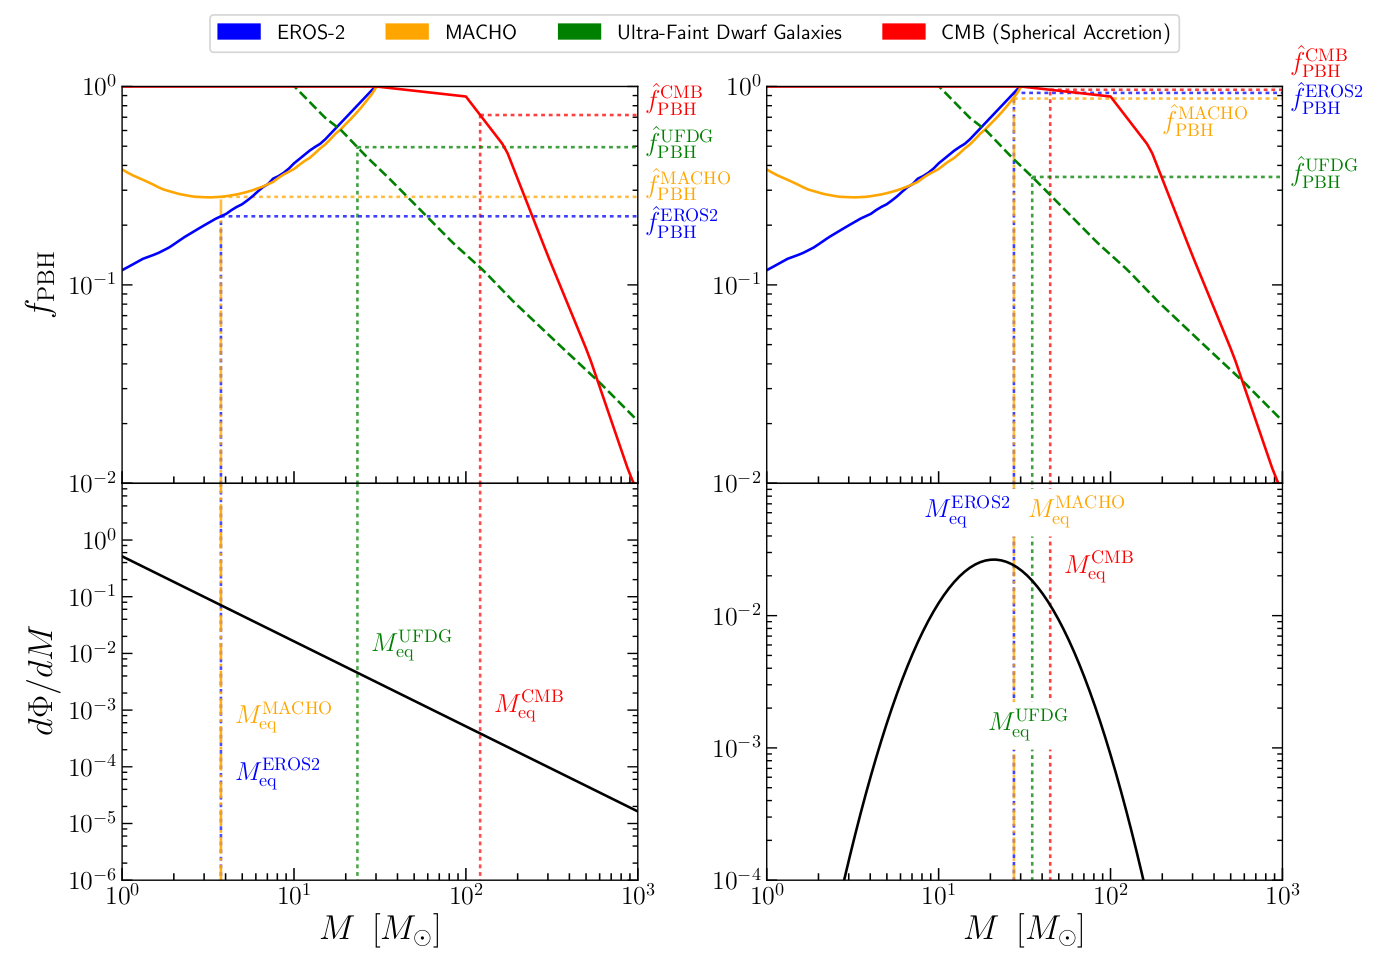
\includegraphics[width=0.7\textwidth]{Bellomo.png}
    \caption{Microlensing(EROS-2, MACHO), ultra-faint dwarf galaxies(UFDG), and cosmic microwave background (CMB) constraints for MMD are shown in the upper panels, respectively. Constraints that are often regarded as being robust to astrophysical assumptions are shown by solid lines, while those whose robustness has not yet been adequately explored in the literature are represented by dashed lines. Lower Panels: Illustrations of lognormal and power law mass distributions, respectively. The vertical dotted lines emphasize the equivalent mass for each observable, and when they connect with the appropriate constraint in the top panels, the set of the maximum permitted  $\hat{f}_{\mathrm{PBH}}$ is retrieved. For the calculation of equivalent masses for each observable refer to Ref.\cite{Bellomo:2017zsr}.\\
    The lowest of the four, or the one determined by EROS2 microlensing (for its matching EM), is the maximum allowable $\hat{f}_{\mathrm{PBH}}^{\mathrm{EROS} 2}$for the PL EMD. On the other hand, the maximum permitted $\hat{f}_{\mathrm{PBH}}^{\mathrm{UFDG}}$ for the selected LN EMD is that given by the UFDG. Figure taken from \cite{Bellomo:2017zsr}  }
    
\end{figure}
This method developed by Bellomo \emph{et al} \cite{Bellomo:2017zsr} enables us to translate MMD to EMD and also compare EMD to MMD constraints. It shows that for any  observable and EMD, there is a corresponding MMD with "Equivalent Mass " producing the same physical and observational effects. They also specified that it is crucial to be cautious of the applicable range of validity when examining observational constraints for EMDs due to the fact that while the assumptions used to describe each observable are normally true for an MMD, they may not always be true for an EMD. Ignoring this may lead to unreliable and even unphysical constraints.\\

In summary, the results show that when utilizing a proper and consistent choice of distribution parameters, a lower abundance of BHs is allowed in extended mass distribution (EMD) models compared to monochromatic mass distribution (MMD) predictions. Specifically, the maximum permissible fraction of dark matter in PBHs within the window where $\hat{f}_{\mathrm{PBH}} \sim 1$ is either displaced or reduced for EMDs.